%                                                                 aa.dem
% AA vers. 9.1, LaTeX class for Astronomy & Astrophysics
% demonstration file
%                                                       (c) EDP Sciences
%-----------------------------------------------------------------------
%
%\documentclass[referee]{aa} % for a referee version
%\documentclass[onecolumn]{aa} % for a paper on 1 column  
%\documentclass[longauth]{aa} % for the long lists of affiliations 
%\documentclass[letter]{aa} % for the letters 
%\documentclass[bibyear]{aa} % if the references are not structured 
%                              according to the author-year natbib style

%
\documentclass[draft]{aa}
% \documentclass{aa}
% \documentclass[referee]{aa}

%
\usepackage{graphicx}
%%%%%%%%%%%%%%%%%%%%%%%%%%%%%%%%%%%%%%%%
\usepackage{txfonts}
%%%%%%%%%%%%%%%%%%%%%%%%%%%%%%%%%%%%%%%%
% To add links in your PDF file, use the package "hyperref"
% with options according to your LaTeX or PDFLaTeX drivers.
%\usepackage[options]{hyperref}
\usepackage{hyperref}
\hypersetup{colorlinks=true, urlcolor=blue, citecolor=cyan, pdfborder={0 0 0}}


\begin{document} 


\title{A complete analysis of NGC2516 with Gaia EDR3 data}
%\subtitle{I. Overviewing the $\kappa$-mechanism}

\author{G.I. Perren \inst{1}\and
M.S. Pera \inst{1} \and
% G. Carraro \inst{2} \and
H. Navone \inst{3,4} \and
R.A. V\'azquez \inst{5}
}

\institute{Instituto de Astrof\'isica de La Plata (IALP-CONICET), 1900 La
Plata, Argentina\\
\email{gabrielperren@gmail.com}
% \and
% Dipartimento di Fisica e Astronomia, Universit\`a di Padova, Vicolo
% Osservatorio 3, I-35122, Padova, Italy
\and
Facultad de Ciencias Exactas, Ingenier\'ia y Agrimensura (UNR), 2000 Rosario,
Argentina
\and
Instituto de F\'isica de Rosario (CONICET-UNR), 2000 Rosario, Argentina,
\and
Facultad de Ciencias Astronómicas y Geofísicas (UNLP-IALP-CONICET), 1900 La
Plata, Argentina
}

   \date{Received XXXXX XX, 2021; accepted XXXX XX, 2021}

% \abstract{}{}{}{}{} 
% 5 {} token are mandatory
 
  \abstract
  % context heading (optional)
  % {} leave it empty if necessary  
   {xxx}
  % aims heading (mandatory)
   {xxx}
  % methods heading (mandatory)
   {xxx}
  % results heading (mandatory)
   {xxx}
  % conclusions heading (optional), leave it empty if necessary 
   {}

\keywords{
  open clusters and associations: general --
  methods: data analysis --
  methods: statistical --
  open clusters and associations: individual: NGC2516
}

   \maketitle



%-------------------------------------------------------------------
\section{Introduction}
 \label{sec:intro}

 The NGC 2516 open cluster (also known as: Melotte 82, Caldwell 96,
 Collinder 172, or Southern Beehive) is a bright cluster visible with the naked
 eye in the southern skies, almost at the center of the Carina constellation.
 It is one of the approximately one hundred cataloged clusters located at a
 distance less than 500 pc away from the solar system.
 Because of its closeness, young age ($\sim 100$ Myr), and clear photometric
 sequence, it has been observed and studied consistently for almost one hundred
 years.
 % The Raab mention is taken from Cox (1955); 10.1086/146028
 \citet{Raab_1922} classified it as a ``very large, thin, irregular,
 well defined cluster containing a very great number of stars, many of which are
 very bright''.
 % Raab quote end with: ``The condensation is conspicuous, but the dispersion
 % unequal.''
 More than 600 references are returned today in a quick SIMBAD bibliography
 search.\footnote{\url{http://simbad.u-strasbg.fr/simbad/}}\\
 
 In Fig.~\ref{fig:ngc2516} we show a Digitized Sky Survey (DSS) frame centered
 on NGC 2516, obtained from the Aladin Sky
 Atlas.\footnote{\url{https://aladin.u-strasbg.fr/}}

 \begin{figure}
 \centering
 \includegraphics[width=\hsize]{figs/NGC2516_DSS.png}
 \caption{NGC 2516, DSS colored image from the Aladin Sky Atlas.}
 \label{fig:ngc2516}
 \end{figure}

 Recently \cite{Borodina_2021} showed that cluster masses increase linearly with
 binary fraction, when binary stars are taken into account. This is: cluster
 masses are underestimated if the presence of binaries is neglected.

 \cite{Kouwenhoven_2009} demonstrated a similar but inverse effect for the
 dynamical masses, i.e. that not taking binary systems into account results in
 an overestimation of the dynamical mass.


 In \citet{Perren_2015}...\\


 This paper is organized as follows: in Section~\ref{sec:data} we
 present the data used in this work. Sections~\ref{sec:structure}
 and~\ref{sec:membership} show the structural and membership analysis,
 respectively.
 xxx
 %
 Results are summarized in Section \ref{sec:results}. Finally, our
 conclusions are given in Section \ref{sec:conclusions}.



%-------------------------------------------------------------------
\section{Gaia EDR3 data}
 \label{sec:data}

 The data used throughout this article is taken from the Gaia EDR3
 survey~\citep{GaiaEDR3_2020}. We downloaded a region of 4x4 deg$^2$ centered
 on $(\alpha_{2016}=119.5167, \delta_{2016}=-60.7533)$, using the
 Vizier\footnote{\url{https://vizier.u-strasbg.fr/viz-bin/VizieR}} service.

 % Why the magnitude cut? Godoy-Rivera et al. (2021):
 % >...G >= 18.5 mag. At this apparent magnitude, instead of continuing to the
 % bottom-right part of the diagram, the probable members start to turn to bluer
 % colors for fainter magnitudes. This feature has already been found by other
 % works when using the Gaia DR2 photometry (e.g., Arenou et al. 2018; Lodieu et
 % al. 2019a,b; Smart et al. 2019), and it arises from an overestimation of the
 % flux in the GBP passband for faint, red sources (Riello et al. 2018, 2020).
 A magnitude cut on $G=18$ mag was imposed on the data resulting in a total of
 114512 sources for the complete frame. Of these, only 882 sources contained
 missing information in either the parallax, proper motions, or photometry,
 and were thus discarded from the fundamental parameters analysis.
 The reason for using only stars with $G\leq18$ mag is that below
 $G\approx18.5$ mag the Gaia color $BP-RP$ starts
 to become more negative, shifting the stars towards a non-physical (bluer)
 region of the color-magnitude diagram (CMD). This effect is attributed
 to an overestimation of the flux in the $BP$ passband for faint
 sources~\citep{Godoy_2021}. This artifact in the photometry would obviously
 have a negative impact on the CMD analysis, presented in
 Sect.~\ref{sec:fund_pars}. In addition, below $G=18$ mag the uncertainties of
 not only the photometry but also the proper motions and parallax start
 exponentially growing to very large values. This cut allows us to keep the
 sub-sample of data with the lowest uncertainties.

 %
 % Completeness Gaia EDR3
 % Fabricius et al. (2020):
 % For bright sources, detection efficiency starts to drop at G~3 mag
 %
 % Gaia Collaboration, Brown, A.G.A., et al.
 % https://doi.org/10.1051/0004-6361/202039657
 % In combination with the still limited data treatment in crowded areas this
 % means that the survey limit in regions with densities above a few hundred
 % thousand stars per square degree can be substantially brighter than G = 20.
 % Fabricius et al. (2020) show that the completeness as measured on OGLE fields
 % is 100\% up to source densities of 2x10^5 deg^-2, while at higher densities the
 % completeness has improved with respect to Gaia DR2, staying close to 100\% up
 % to 6x10^5 stars deg^-2 and dropping to 50\% at densities over
 % 8x10^5 deg^-2
 As shown in~\cite{Fabricius_2020}, a 100\% completeness of Gaia EDR3 data is
 guaranteed up to $G=20$ mag for regions of density below $2\times10^5$
 deg$^{-2}$. Our downloaded Gaia EDR3 frame containing NGC 2516 has a maximum
 density that is smaller than $\sim1.1\times10^5$ deg$^{-2}$ at its peak.
 Hence, this guarantees that the studied cluster sequence is complete down to
 the lowest-mass stars. This is an important fact to establish, since the
 estimated total cluster mass depends heavily on the total number of
 identified true  members.\\

 \begin{figure*}
 \resizebox{\hsize}{!}{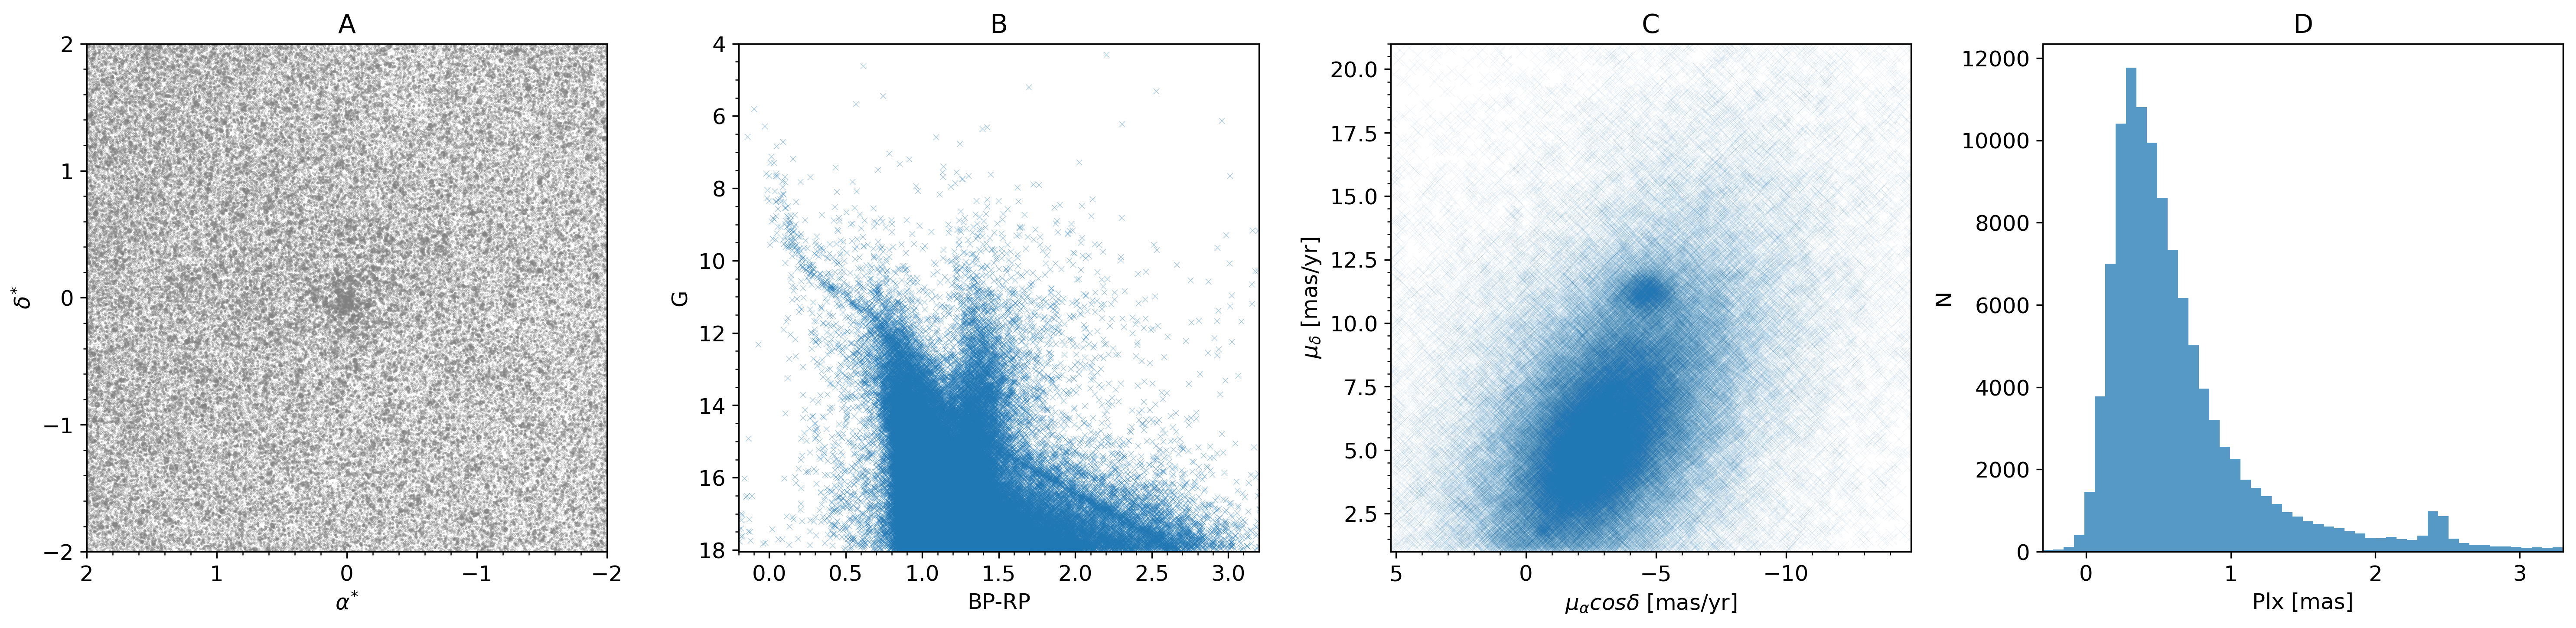
\includegraphics{figs/NGC2516_4_plots.png}}
 \caption{A: (transformed) right ascension and declination for the full frame.
 B: CMD for all the sources.
 C: vector-point diagram (VPD) for the proper motions, centered and zoomed on
 the cluster's estimated systemic values.
 D: Histogram of the parallax values, in the range [-0.5, 3.5] mas.}
 \label{fig:ngc2516_4}
 \end{figure*}

 In Fig.~\ref{fig:ngc2516_4} we show the final Gaia EDR3 data analyzed in this
 work. The $(\alpha^{*}, \delta^{*})$ coordinates are displaced to the
 cluster's center, and the right ascension is multiplied by the cosine of the
 declination. In all four plots the position of the cluster visibly stands out
 from the remaining field stars.




%-------------------------------------------------------------------
\section{Structural properties}
 \label{sec:structure}
 
 The region surrounding this cluster shows a markedly non-uniform distribution
 of field stars. This contamination appears mostly above $G\approx15$ mag, as
 seen in~Fig\ref{fig:density}.

 \begin{figure}
 \centering
 \includegraphics[width=\hsize]{figs/dens_map.png}
 \caption{Density maps of the NGC 2516 frame, $N$ is the number of stars in
 each plot. Left: complete frame. Center: stars brighter than $G=15$ mag. Right:
 low mass stars below $G=15$ mag.}
 \label{fig:density}
 \end{figure}

 To estimate the radius we employed our \texttt{ASteCA}
 package~\citep{Perren_2015} to fit a King profile\citep{King_1962}, for stars
 up to $G=15$ mag.
 \cite{Pieres_2016}



%-------------------------------------------------------------------
\section{Membership analysis}
 \label{sec:membership}

 In this section we present the membership estimation method and the final set
 of most likely member stars.

 A first coarse manual estimation of the total number of members was performed
 with the \texttt{glue} library\footnote{\url{http://glueviz.org/}}. This
 application allows the selection of a subset of data, linked throughout
 multiple dimensions. The process is as follows: we begin by selecting the
 clearly visible overdensity of stars in the space of proper motions. These are
 then filtered using the parallax dimension, keeping stars that don't deviate
 too much from the mean. Finally, the subgroup is filtered again in the
 coordinates space, to keep stars within 1.5 deg from the cluster's center 
 (the estimated radius, as explained in Sect.~\ref{sec:structure}).
 This simple method results in a group of approximately 1400 stars
 manually selected to be the most likely members.

 A second simple estimation 



  \begin{figure}
  \centering
  \includegraphics[width=\hsize]{figs/dens_vs_rad.png}
  \caption{Density estimation versus distance to the center of NGC 2516.}
  \label{fig:dens_vs_rad}
  \end{figure}






%-------------------------------------------------------------------
\section{Estimation of fundamental parameters}
 \label{sec:fund_pars}

 xxx


  %****************************************************************
  \subsection{Fundamental parameters with \texttt{AsteCA}}
   \label{ssec:asteca}



  %****************************************************************
  \subsection{Identification of single/binary systems}
   \label{ssec:id_single_binaries}

   xxx
   
   % Valle et al. (2021), "Goodness of fit test...", Describes a two-step
   % process to identify binary systems, based on rejecting stars far away
   % from a fiducial line estimated in the CMD
   %
   % In OCs an average fraction of binaries of about 30\% (i.e. η = 0.3) is
   % expected  (see e.g. Gizis & Reid 1995; Bouvier et al. 2001; Böhm-Vitense
   % 2007; Boudreault et al. 2010; Khalaj & Baumgardt 2013; Sheikhi et al.
   % 2016; Borodina et al. 2019; Li et al. 2020)

    % Rubele et al. (2011):
    % https://academic.oup.com/mnras/article/414/3/2204/1038836
    % The binary fraction is set to a value of 0.3 for binaries with mass ratios in
    % the range between 0.7 and 1.0, which is consistent with the prescriptions for
    % binaries commonly used in works devoted to recover the field SFH in the
    % Magellanic Clouds (e.g. Holtzman et al. 1999; Harris & Zaritsky 2001; Javiel,
    % Santiago & Kerber 2005; Noel et al. 2009). Notice that this assumption is
    % also in agreement with the few determinations of binary fraction for stellar
    % clusters in the LMC (Elson et al. 1998; Hu et al. 2010, both for NGC 1818, a
    % stellar cluster younger than ∼100 Myr).

    % [Arenou et al. 2018](https://doi.org/10.1051/0004-6361/201833234) also
    % proposes a simple method to identify binaries:
    %
    % Binary stars were first selected and removed. We used a LOWESS fitting 
    % (Cleveland 1979) to follow the sequence, and removed binary star
    % candidates by clipping out sources with G_BP fluxes two error bars lower
    % and G_RP fluxes higher than the fitted relation.
    %
    % Cleveland 1979: https://api.semanticscholar.org/CorpusID:31665444

    % Borodina et al. (2021) https://api.semanticscholar.org/CorpusID:230524157
    % If not properly accounted for, unresolved binary stars can induce a bias
    % in the photometric determination of star cluster masses inferred from star
    % counts and the luminosity function

    Sollima et al. (2010) estimated a 66\% binary fraction, with a minimum of
    25\%. These are values for the core of the cluster.

    % Belokurov et al (2020) https://ui.adsabs.harvard.edu/abs/2020MNRAS.496.1922B/abstract
    % For stars with unresolved companions, motions of the centre of light and
    % that of mass decouple, causing a single-source astrometric model to
    % perform poorly. We show that such stars can be easily detected with the
    % RUWE
    %
    % Bouma et al (2021)
    % To assess astrometric binarity, we used the renormalized unit weight error
    % (RUWE) from Gaia EDR3. For plotting purposes, we labeled anything with
    % RUWE exceeding 1.2 as an astrometric binary (11% of the overall cluster
    % sample; see e.g., Belokurov et al. 2020). To assess photometric binarity,
    % we fitted a spline to Figure 3, fixing the nodes by hand. We then labeled
    % any points brighter than 0.3 mag above the cluster sequence as photometric
    % binaries. This included 20% of the overall cluster sample.
    %
    % They find a binary fraction in the range 11%-20%
    %
    Using the RUWE statistic, the binary fraction estimated as Bouma et al 
    (2021) (i.e., RUWE>1.2) is around $\sim$14\%.



  %****************************************************************
  \subsection{Estimation of masses for binary systems}
   \label{ssec:mass_binaries}


   In \cite{Borodina_2021} the authors use a quadratic mass-luminosity relation
   for main sequence stars, to estimate the masses for the primary and secondary
   stars in a binary system.


%-----------------------------------------------------------------
\section{Results}
 \label{sec:results}

 % Mass segregation:
 % ---------------------------------
 \cite{Jeffries_2001}
 % We conclude that the evidence for mass segregation is strong when comparing
 % stars above and below about ~0.8 Mo
 %
 % This is perhaps a hint that at least some of the mass segregation in NGC 2516
 % is primordial, as has been supposed for some younger clusters (...) cluster
 % relaxation timescale - which is about 100 Myr for clusters of the size of NGC
 % 2516 



 % Binarity & Mass
 % ---------------------------------
 \cite{Gonzales_2000}
 % A binary frequency of more than 26% is found among the high-mass
 % main-sequence stars. This number rises to 46% if all suspected binaries are
 % included.


 \cite{Jeffries_2001}
 % binary fraction of 26+/-5% ; binary fraction estimated in this way is a lower
 % limit.
 % "mass segregation is clearly present"
 % "the total cluster mass might be significantly greater than just what we
 % have observed in our limited survey"
 % "The total mass of the cluster for stars with M>0.3 M is at least 950 M and
 % probably as high as 1200 M, depending on the metallicity, binary fraction
 % and mass-ratio distribution. Correcting for the fraction of stars that lie
 % outside our survey, but within the likely cluster tidal radius, may increase
 % this estimate to around 1240-1560"
 % "less massive stars and brown dwarfs contribute about a further 15 percent
 % to the mass of NGC 2516"
 % 
 % "We must provide a caveat here; our selection procedure is arbitrary to some
 % degree, and will exclude some genuine members and will include some
 % non-members"
 %
 % The total cluster mass is probably greater than we first estimated (...)
 % likely that the cluster is more massive by about a factor of 1.3.
 %
 % Combining the upper mass limit (1560) with the projection of 15% more mass
 % from low mass stars, I get ~1800 as the upper mass limit
 %
 % Healy & McCullough(2020) quote the mass range from Jeffires as: 1240-1560 Mo

 \cite{Sung_2002}
 % dm=7.77, E_BV=0.122, log(age)=8.2, [FE/H]=-0.1, b_fr=40% (minimum)
 %
 % Jeffries, Thurston, & Pye 1997: [Fe/H]=-0.32
 % Jeffries, James, & Thurston 1998 could reach no definite conclusion (for the)
 % metallicity
 %
 % "One of important issues concerning NGC 2516 is its metallicity: is it sub-
 % or near-solar?"

 \cite{Bonatto_2005}
 % NGC 2516: Battinelli et al. (1994) give Rlim ≈ 1.9 pc and
 % mtot ≈ 282 M. Bergond et al. (2001) give d ≈ 0.4 kpc, an
 % age of ≈113 Myr, Rtidal = 1.9 pc and mtot ≈ 170 M. Tadross
 % et al. (2002) give d ≈ 0.4 kpc, age ≈ 63 Myr, Rlim ≈ 1.8 pc,
 % dGC ≈ 8.5 kpc and mtot ≈ 36 M. Jeffries et al. (2001) estimate
 % an age of ≈150 Myr and total mass of mtot ≈ 1240−1560 M.
 % They also detected a sharp change in the MF slope for stars
 % with 0.3 ≤ m(M) ≤ 0.7.
 %
 % We note that previous works gave exceedingly low values for the
 % stellar mass in NGC 2516, e.g. Bergond et al. (2001) estimate
 % mtot ≈ 170 M (for stars with m ≥ 1.1 M), while in Tadross
 % et al. (2002), mtot ≈ 36 M.
 %
 % in the present work mtot = 1280 ± 162 M


 \cite{Piskunov_2007}
 % Dist E(B-V)   logt    r1     r2    N2   rc    rt     k    logM
 %   pc    mag   [yr]   deg    deg         pc    pc          [solMass]
 % 346    0.07   8.08  0.20   0.70    31  1.9   7.1   4.3    2.126


 \cite{Piskunov_2008}
 % DistMod  E(B-V)   Dist    logt     rt       logM      rtA     logMA
 %   mag      mag     pc     [yr]     pc    [solMass]    pc    [solMass]
 % 7.912     0.07    346     8.08    8.6      2.369      8.7      2.396
 %
 % rtA: Tidal radius derived from semi-major axis A
 % logMA: Log of Cluster mass from semi-major axis A  


 \cite{deGrijs_2008}
 % log(age)=8.2 ; Dynamical Mass: 3970 +/- 1680
 %
 % NGC 2516 is presently located some 120 pc below the Galactic plane, near the
 % dense molecular clouds of the Vela Sheet. These Galactic plane
 % passages may have contributed to rendering the cluster unstable.
 % Alternatively, encounters with giant molecular clouds (e.g.,
 % Gieles et al. 2006), particularly around the time of Galactic plane
 % passages, may have contributed to the cluster’s present dynamical state.

 \cite{Kouwenhoven_2009}
 % dynamical mass of a star cluster with a low binary fraction is expected to
 % be only barely overestimated

 \cite{Jilinski_2009} analyzes the orbit
 % "The total mass of NGC 2516 is presently not well known"

 \cite{Silai_2014}
 % Age and metallicity estimates

 \cite{Liu_2019}
 % Liu et al. (2019)
 % rmax: Maximum cluster member's distance to average position 
 % nTot: Total number of stars in primary sample
 % rmax     plx     e      pmRA     e      pmDE     e     nTot    Age     e       Z  
 % deg     mas    mas    mas/yr mas/yr   mas/yr mas/yr           Gyr    Gyr    [Sun]
 % 2.295   2.409  0.067   -4.661  0.521   11.170  0.438   1415   0.093  0.0056   0.25


 \cite{Jackson_2016}


 \cite{Jackson_2020}


 \cite{Pang_2021}
 % Pang et al. (2021)
 %  rh and rt are half-mass and tidal radii 
 % Age Distcor  rh     rt    Mcl   Mdyn      Z  E(B − V ) Nmemb CG20  LP19
 % 123   410.5  7.9  18.3  1973.3 3368.2  0.020   0.05     2690  640  1365

 % Mcl is the total mass of the star cluster (i.e., the sum of the masses of the
 % individual member stars)
 % mass of each individual member star is obtained from the nearest point in the
 % fitted isochrone

 %
 % An extended main sequence turn-off (eMSTO) of $\sim$0.3 mag in the color
 % GBP-GRP is observed in (...) NGC2516

 % dynamical masses (are) higher than the estimated photometric masses ...
 % suggest the majority of clusters might be supervirial

 % No evidence for mass segregation is found (using the Lambda method)


 \cite{Cantat-Gaudin_2020}
 % Cantat-Gaudin et al. (2020), 640-A1
 % r50: Radius containing half the members <-- Says 'arcsec' but must be deg
 % nbstars07: Number of members with proba over 0.7  
 % AVNN: DMNNExtinction Av of the cluster  
 % DMNN: Distance modulus of the cluster  
 %   r50 nbstars07  pmRA*    pmDE    plx  AgeNN AVNN  DMNN
 % 0.496       652 -4.748  11.221  2.417   8.38 0.11  8.14

 % READ
 % IMF: 'The Origin of the Initial Mass Function', Bonnell (2006)


 \cite{Borodina_2021}
 % cluster masses increase when binary stars are appropriately taken into account


 \cite{Spina_2021}
 % metallicity: [Fe/H]=-0.079+/0.025 (N=2)
 % clusters' iron abundances [Fe/H] are derived from stellar members with ΔTeff
 % <150 K and spectra of SNREV ≥100 (APOGEE) and snr_c2_iraf ≥50 (GALAH). In
 % addition, we apply a 3-sigma clipping before calculating the median [Fe/H]
 % and standard deviation of each cluster population
 %
 % Stars with [Fe/H] (Table 3):
 % RAJ2000 DEJ2000 GALAH [Fe/H]  e_[Fe/H]
 % 120.6408997 -61.0068092 161212004101026 0.114 0.159
 % 118.4987869 -60.8221283 161212004101190 0.106 0.175
 % 119.6553879 -60.5938606 161212004101327 0.104 0.133
 % 118.5264053 -60.7309189 161212004101206 0.083 0.146
 % 119.3177261 -60.7870522 151231003701036 0.064 0.141
 % 120.0207291 -60.5589409 161212004101330 0.051 0.115
 % 118.5475998 -60.4100876 151231003701363 0.035 0.108
 % 120.6507797 -60.7564507 161212004101394 0.034 0.132
 % 120.199913  -60.8656311 161212004101018 0.031 0.069
 % 120.2862549 -60.4763603 161212004101344 0.014 0.123
 % 118.6808624 -60.4120674 161212004101242 0.008 0.095
 % 119.5218353 -60.7944756 151231003701026 0.006 0.122
 % 119.1837616 -60.5811272 161212004101252 0.004 0.068
 % 118.884758  -60.3858871 161212004101253 -0.022  0.078
 % 117.706459  -60.0787392 140307001101101 -0.03 0.116
 % 119.2540359 -60.1960144 151231003701376 -0.035  0.118
 % 119.4002838 -60.8034859 161212004101139 -0.036  0.084
 % 118.5485077 -60.7999725 161212004101193 -0.039  0.091
 % 118.7746048 -61.0748138 161212004101152 -0.042  0.069
 % 119.3542862 -60.6547737 151231003701018 -0.055  0.091
 % 118.5645981 -60.9688225 161212004101171 -0.069  0.111
 % 120.0393295 -60.5598412 161212004101352 -0.069  0.068
 % 120.4023514 -60.9838829 161212004101031 -0.073  0.079
 % 119.6773224 -60.6721535 161212004101349 -0.077  0.071
 % 119.1796112 -60.9096375 151231003701052 -0.095  0.12
 % 119.6452026 -61.053299  161212004101079 -0.104  0.054




%-----------------------------------------------------------------
\section{Conclusions}
 \label{sec:conclusions}

 xxx





\begin{acknowledgements}
 This research has made use of the SIMBAD database, operated at CDS,
 Strasbourg, France~\citep{Wenger_2000}.
 %
 This research has made use of the VizieR catalogue access tool, CDS,
 Strasbourg, France (DOI: 10.26093/cds/vizier). The original description of
 the VizieR service was published in \cite{Ochsenbein_2000}.
 %
 This research has made use of ``Aladin sky atlas'' developed at CDS,
 Strasbourg Observatory, France \citep{Bonnarel_2000,Boch_2014}.
\end{acknowledgements}


\bibliographystyle{aa}
\bibliography{biblio}

\end{document}
